\documentclass[a4paper, 12pt]{extreport}  %размер бумаги устанавливаем
%А4, шрифт 14пунктов
\usepackage{amssymb,amsfonts,amsmath,mathtext,cite,enumerate,float} %подключаем нужные пакеты расширений
\usepackage[pdftex,unicode]{hyperref}
\usepackage[T2A]{fontenc}
\usepackage[utf8]{inputenc}%включаем свою кодировку: koi8-r или utf8 в UNIX, cp1251 в Windows
\usepackage[english,russian]{babel}%используем русский и английский языки с переносами
\usepackage{graphicx} %хотим вставлять в диплом рисунки?
\usepackage{graphics}
\usepackage{colortbl}
%\usepackage{cyrtimes}
\usepackage{color}
\usepackage{multirow}
\usepackage{url}
\usepackage[labelsep=period,justification=centering]{caption}
\usepackage[onehalfspacing]{setspace}  % 1,5 интервал
\usepackage[a4paper]{geometry}
 \geometry{ left=15mm, right=15mm, top=15mm, bottom=15mm}

\DeclareCaptionLabelFormat{figurelabelformat}{\textit{#1~#2}}
\captionsetup[figure]{labelformat=figurelabelformat}

\bibliographystyle{unsrt}
\makeatletter
\renewcommand{\@biblabel}[1]{#1.} % Заменяем библиографию с квадратных скобок на точку:

\begin{document}
\begin{flushleft}
{\bf УДК 519.688}
\end{flushleft}
\begin{center}
\textbf{{Разработка методов трекинга для эксперимента BM@N на Нуклотроне ОИЯИ}}
\newline

П.Н.~Батюк, С.П.~Мерц\footnote{Sergey.Merts@gmail.com}, Г.А.~Ососков, О.В.~Рогачевский
\newline 

Дубна, Объединенный Институт Ядерных Исследований (ОИЯИ)
\end{center}

При получении информации в экспериментах физики высоких энергий необходимым и
важным этапом является реконструкция событий взаимодействия сталкивающихся
частиц: нахождение треков частиц и их параметров, затем, с использованием этой
информации - вершин событий. Для решения этой задачи обычно используется 
математический аппарат, основанный на фильтре Калмана. Применение этого аппарата
требует перебора большого числа реконструированных откликов детектора на
прохождение через него частиц, необходимого для получения начальных приближений
параметров треков заряженных частиц (нахождение треков-кандидатов). В данной
работе представлен новый подход к решению задачи реконструкции, значительно
снижающий комбинаторику (число переборов хитов).
\newline

Фильтр Калмана, трекинг, эффективность трекинга, преобразование координат

%\newpage
\section*{Эксперимент BM@N}

В соответствии с планами исследований образования плотной барионной материи на
ускорительном комплексе «Нуклотрон-М»  планируется создание и последующая
эксплуатация экспериментальной установки BM@N (Baryonic Matter at
Nuclotron)~\cite{bmn}. Данная установка относится к классу установок с
фиксированной мишенью. Физическая программа планируемого эксперимента
предполагает изучение странной материи, образующейся при столкновениях тяжелых
ионов в широком энергетическом диапазоне вплоть до энергий порядка 4 ГэВ/нуклон.

На рисунке~\ref{img:bmn} представлено схематическое изображение
экспериментальной установки BM@N. Основным трековым детектором в эксперименте
являются 12 плоскостей, составленных из газовых электронных умножителей (GEM),
помещенных в дипольный магнит. За пределами магнита располагаются две дрейфовые
камеры (DCH1, DCH2), два времяпролетных детектора (TOF1, TOF2) и калориметр
(ZDC). 

\begin{figure}[h!]
\center{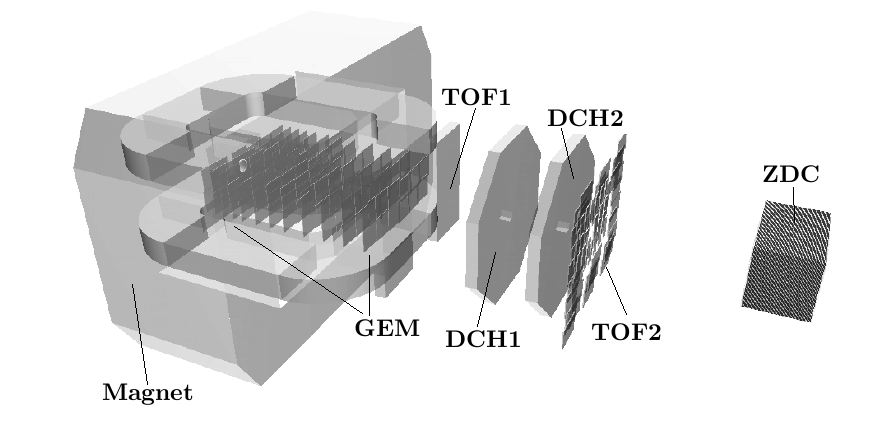
\includegraphics[width=1.0\linewidth]{bmn.png}}
\caption{Схематический вид экспериментальной установки.}
\label{img:bmn}
\end{figure}

Для изучения возможностей этой установки необходимо провести моделирование
составляющих ее детекторных подсистем (подробное описание всей геометрии, параметризация
физических процессов, происходящих в детекторных подсистемах во время работы и
пр.), разработать и отладить методы и алгоритмы реконструкции событий. На
данном этапе разработки проекта именно оценки точности получаемых физических
параметров и качества реконструкции позволяют оптимизировать структуру
детектора.  

\section*{Восстановление треков заряженных частиц}

Общепризнанным методом реконструкции треков заряженных частиц в подобных
установках является алгоритм калмановской фильтрации~\cite{kf1, kf2},
скорость работы которого сильно зависит от способа выбора начальных приближений
(треков-кандидатов). Выбор делается посредством перебора всех возможных комбинаций 
реконструированных откликов детектора на прохождение через него частиц (далее хитов), 
что в случае событий с высокой множественностью заряженных частиц сильно увеличивает 
вычислительную сложность задачи~\cite{timur}.

\begin{figure}[h!]
\center{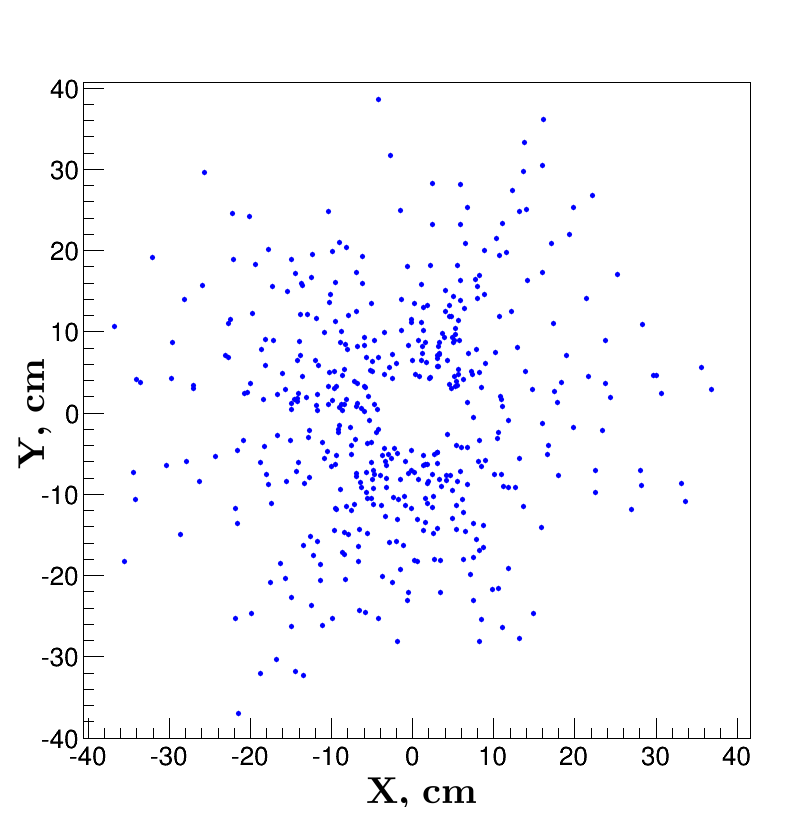
\includegraphics[width=0.5\linewidth]{yx.png}}
\caption{Распределение хитов в пространстве $\{x, y\}$.}
\label{img:xRyR}
\end{figure}

В данной работе для поиска треков-кандидатов использовались хиты, полученные с 
первых пяти GEM-станций. Магнитное поле предполагалось однородным и имеющим
только y-компоненту, равную по абсолютному значению 9 кГс.

На рисунке~\ref{img:xRyR} представлен пример распределения хитов в
пространстве $\{x, y\}$, полученный путем моделирования в программном комплексе
BmnRoot~\cite{bmnroot} прохождения заряженных частиц через детектор BM@N. 

Группировка хитов, относящихся к одному треку, в случае высоких множественностей
частиц представляет сложную вычислительную задачу. В представленной работе
предложен метод, существенно снижающий комбинаторную сложность задачи.

\begin{figure}[h!]
\center{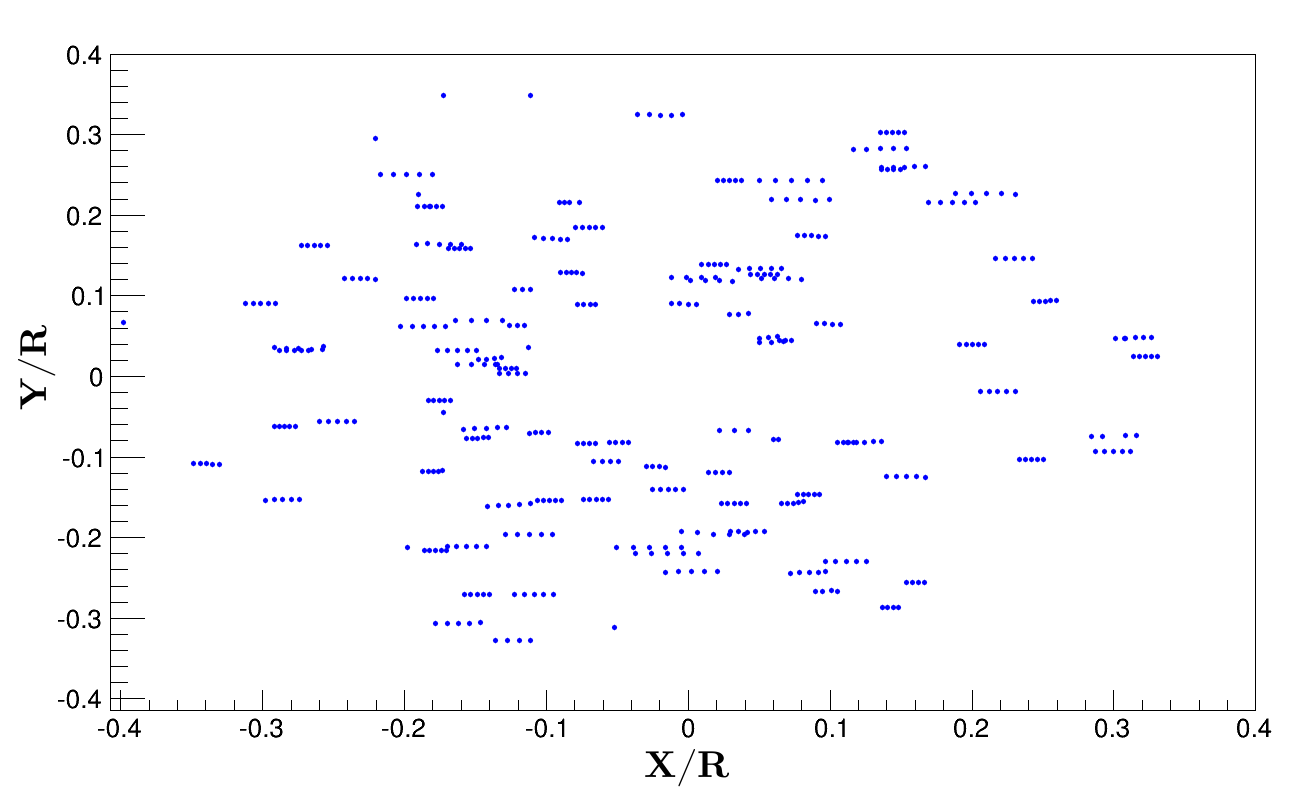
\includegraphics[width=0.75\linewidth]{yRxR_new.png}}
\caption{Распределение хитов в пространстве $\{\frac{x}{R}, \frac{y}{R}\}$.}
\label{img:xRyR1}
\end{figure}

\section*{Координатное преобразование хитов} 

Предложенный в работе метод поиска треков-кандидатов основывается на следующем
отображении декартовых координат хитов:

$$\{x, y\} \longmapsto \{\frac{x}{\sqrt{x^2 + y^2 + z^2}}, \frac{y}{\sqrt{x^2 +
y^2 + z^2}}\}$$

В результате данного отображения треки частиц преобразуются в короткие
горизонтальные отрезки, в которых расстояние между хитами зависит от импульса:
чем больше импульс, тем ближе расположены хиты (см.~Рисунок~\ref{img:xRyR1}).

После применения данного преобразования решение задачи поиска треков-кандидатов
сводится к следующему алгоритму:
\begin{enumerate}

\item Каждому хиту приписывается вес $\omega_i$ равный номеру GEM-станции.

\item В распределении из рисунка~\ref{img:xRyR1} осуществляется поиск хитов с весом
$\omega = 1$.

\item Выполняется поиск соседних хитов слева и справа, удовлетворяющих 
условию~$\omega_i > \omega_{i-1}$.

\item Критерием прекращения поиска служит условие $|\frac{X_i}{R_i} -
\frac{X_{i-1}}{R_{i-1}}| > N \cdot D_{max}$ где $D_{max}$ -- максимальное
расстояние между найденными хитами, $R_i = \sqrt{x_i^2 + y_i^2 + z_i^2}$ --
радиус-вектор хита, $N = 4$ -- масштабный фактор, задающий ширину коридора
поиска хитов.

\item Найденные хиты аппроксимируются окружностью с помощью метода быстрой
робастной подгонки~\cite{circ1, circ2}.

\item Из параметров полученных окружностей и наклона геликоид вычисляются
необходимые для алгоритма калмановской фильтрации компоненты вектора состояния и
ковариационной матрицы.

\item Хиты, не прошедшие отбор при аппроксимации (п.~5), возвращаются в
общий массив для повторной обработки.
\end{enumerate}

В результате работы алгоритма создается массив треков-кандидатов, которые и
являются начальными приближениями для трекинга с использованием фильтра Калмана.

\section*{Результаты}

Разработанный алгоритм был протестирован на данных, смоделированных для
эксперимента BM@N. Эффективность работы алгоритма представлена на
рисунке~\ref{img:efficiency}.

В качестве величин, показывающих эффективность трекинга и процент ложно
определенных треков, выбраны следующие:

$$Eff = \frac{N_{found}}{N_{gen}} \cdot 100\%$$
$$Ghost = (1 - \frac{N_{well}}{N_{gen}}) \cdot 100\%$$

где $N_{gen}$ -- общее число смоделированных треков, $N_{found}$ -- общее число
найденных треков, $N_{well}$ -- число треков, у которых более 70\% хитов
являются присоединенными к треку верно.

\begin{figure}[h!]
\center{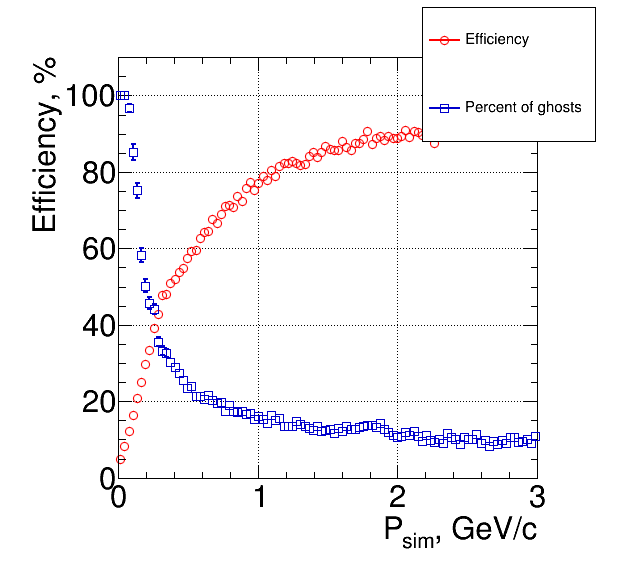
\includegraphics[width=0.65\linewidth]{efficiency.png}}
\caption{Эффективность распознавания треков.}
\label{img:efficiency}
\end{figure}

Высокое значение числа ложных треков (ghosts) в диапазоне импульсов до 1~ГэВ/с
обусловлено жестким условием на определение $N_{well}$.

Предложенный метод поиска треков-кандидатов существенно уменьшает число
переборов хитов и совместно с использованием фильтра Калмана показывает высокую
эффективность реконструкции для широкого диапазона импульсов.

Импульсное разрешение (см.~рисунок~\ref{img:res}) реконструированных треков не
превосходит 3\% для широкого диапазона импульсов, что также говорит о высоком
качестве реконструкции событий.

\begin{figure}[h!]
\center{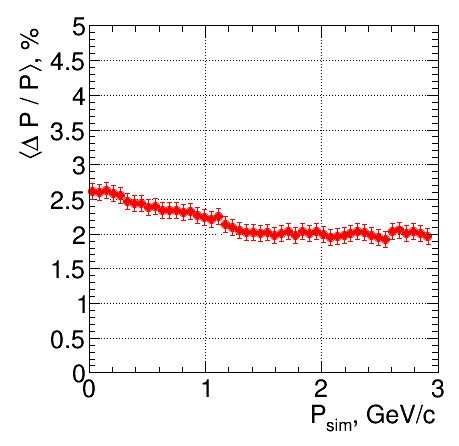
\includegraphics[width=0.65\linewidth]{Mom_res.png}}
\caption{Импульсное разрешение восстановленных треков.}
\label{img:res}
\end{figure}

\begin{thebibliography}{99}
	\bibitem{bmn}BM@N collaboration. BM@N proposal for JINR-PAC. //
JINR-PAC Meeting in January, 2012. 28~p.
	\bibitem{kf1}Fruehwirth~R. // Nucl. Instrum. Meth. 1987. A262.
	\bibitem{kf2}Lebedev A., Ososkov G. Track reconstruction in the CBM
TRD~// JINR Communication E10. Dubna. 2008.
	\bibitem{timur} Ablyazimov T.~O., Zyzak M.~V., Ivanov V.~V., Kisel P.~I. // Pis'ma v
ECHAYA. V.~11, №~4 (188), 2014. Pp.~828-846. [in Russian]
	\bibitem{bmnroot}BmnRoot framework. http://mpd.jinr.ru
	\bibitem{circ1}Chernov N.I., Ososkov G.A. // J. of Computer Physics Communications. V.~33. 1984. Pp.~329-333.
	\bibitem{circ2}Ososkov G.A., Polyansky A., Puzynin I.V. // ECHAYA., V.~33. №.~3. 2002. Pp.~676-741. [in Russian]
\end{thebibliography}

\newpage

{\bf Development of methods for tracking in the BM@N experiment at Nuclotron of the Joint Institute for Nuclear Research (JINR)}
\newline

Batyuk P.~N., Merts S.~N.\footnote{Sergey.Merts@gmail.com}, Ososkov G.~A., Rogachevsky O.~V.
\newline

Russia, Dubna, Joint Institute for Nuclear Research
\newline

Event reconstruction of interactions of the colliding particles aimed to reconstruct tracks
of particles and their parameters, and, subsequently, parameters of vertices is an issue that seems
to be very important in the high energy physics. A special mathematical technique based on the
Kalman filter is used to fulfill the event reconstruction procedure. However, it requires a
tremendous search of the reconstructed responses of a detector on the particles passing aimed to obtain
initial approximations of the track parameters of charged particles. In the current paper an original
approach to the event reconstruction is presented which allows for decreasing combinatorics considerably.
\newline

Kalman filter, tracking, efficiency of tracking, transformation of coordinates

\end{document}


